In finite element modeling, a finer mesh usually results in a more accurate solution. However, as a mesh is made finer, the computation time increases. To get a mesh that satisfactorily balances accuracy and computing resources, a mesh convergence study has to be performed.

In this scope, the breast and muscle geometries were meshed with different mesh sizes; the minimal elements sizes was set to $7mm$ and the maximal element size was varied to $\lbrace 7mm$,  $10 mm$, $13mm$, $15mm$, $17mm$, $20mm\rbrace$. Simulation with a mesh size of $5mm$ was not supported as it become too expensive in computation time and memory therefore a computer with higher computational power was needed.  The compression paddle geometries were meshed with a constant element size of $1mm$. The number of elements obtained for each mesh size is given in Table  \ref{nbElementsvsmeshsize}. We can see that, in general, larger the mesh size, lower the number of elements. However, we observed that for a mesh size equal to 17 mm, a higher number of elements was obtained when compared to a mesh size of 15mm. This is due to the fact that the mesh size being defined by the maximal and minimal elements size, a higher number of \textit{small} elements is needed to cover the areas smaller than the \textit{large} elements. With such meshes, the element density is usually concentrated on the corners or narrow spaces which, in our case, do not coincide with the region of interest.  

\begin{table}[!h]
\begin{tabular}{|c|c|c|c|c|c|c|}
\hline
Mesh size & 20mm & 17mm & 15mm & 13mm & 10mm & 7mm \\
\hline
Nb. of elements & 8367 & 10897 & 8099 & 10751 & 18453 & 65785 \\
\hline
\end{tabular}
\caption{Number of elements obtained for each mesh size.}
\label{nbElementsvsmeshsize}
\end{table} 

Our model was developed to compute breast deformation under compression, an equivalent simulation was performed to estimate the optimal mesh size. Starting from the breast supine geometry, the gravity was applied in the posterio-anterior direction. Then, the right breast was compressed between the breast support and the paddle (Figure \ref{fig:meshconvergence}). In this work we are interested in tissue deformations, therefore the strain range for each mesh density was analysed. The strain distribution over the breast volume for each mesh size are given in Figure \ref{fig:meshconvergence}. 

\begin{figure}[!h]
\centering
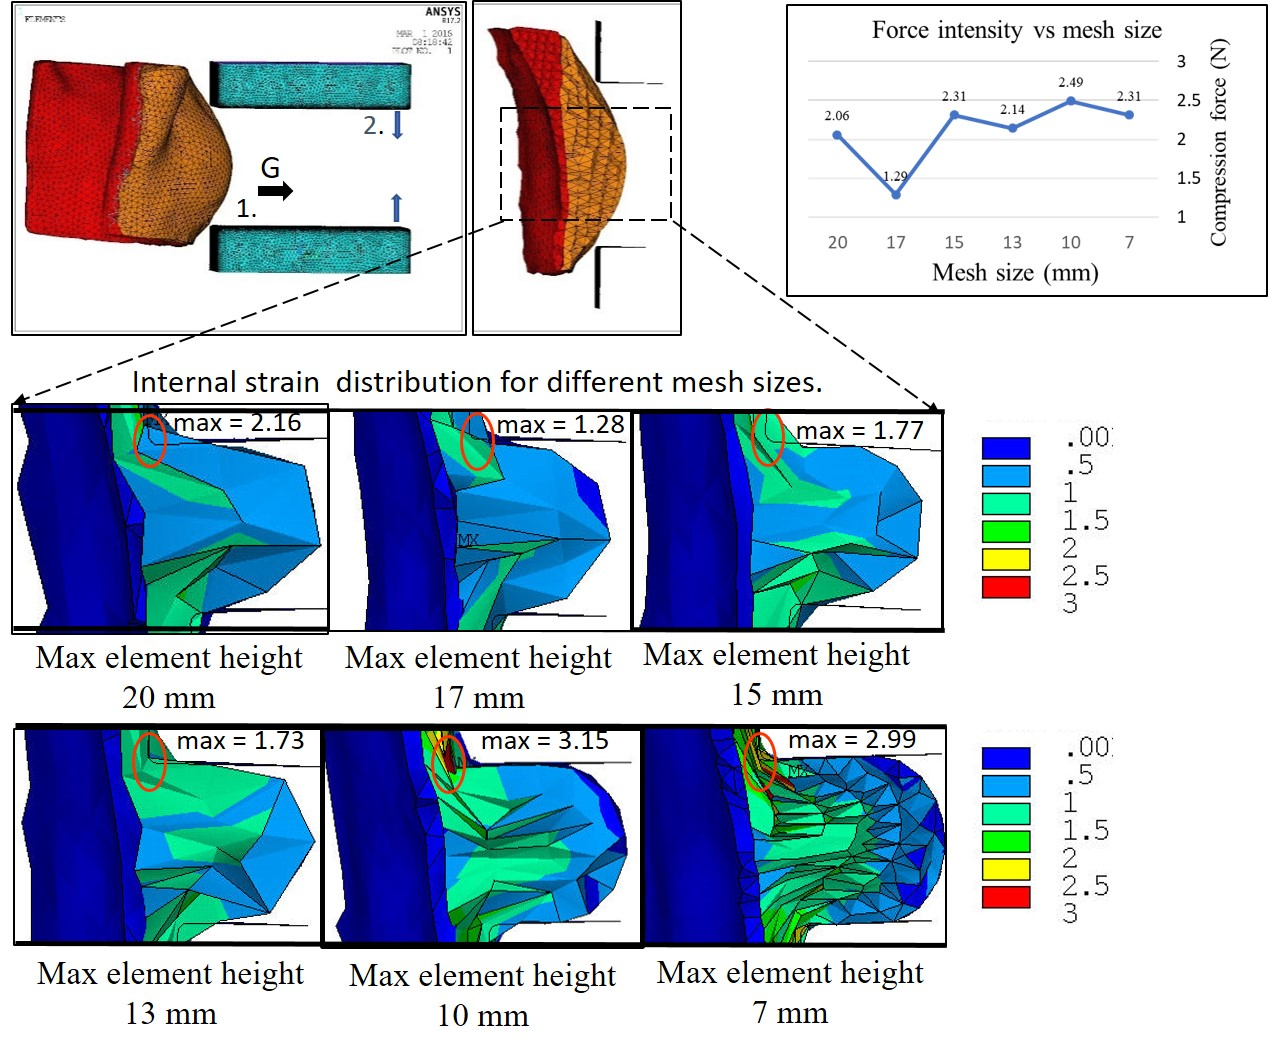
\includegraphics[width=\textwidth,keepaspectratio]{figures/meshConvergence.jpg} 
\caption{Internal strain distribution in function of the elements size. }\label{fig:meshconvergence}
\end{figure}

Under compression, the maximal strain is expected to occur in the juxtathoracic area at the contact with the paddle corner (marked area with an orange ellipsoid in Figure \ref{fig:meshconvergence}), therefore the maximal strain was measured in this region for each mesh density. However, the observed values did not show a converging behavior within different mesh sizes. To analyze the mesh convergence, the applied force for a target compressed breast thickness was plotted (Figure \ref{fig:meshconvergence}). One can see that the force intensity converges starting with a mesh size equal to $15mm$. However, a visual analysis of the strain distributions over the breast volume shows that using a mesh size equal to or lower than 10 mm results in a better estimation of the internal strain distribution. Therefore, to optimize the computation time, a mesh size equal to $10mm$ is used.
